\begin{figure}[h!tp]
  \begin{center}
    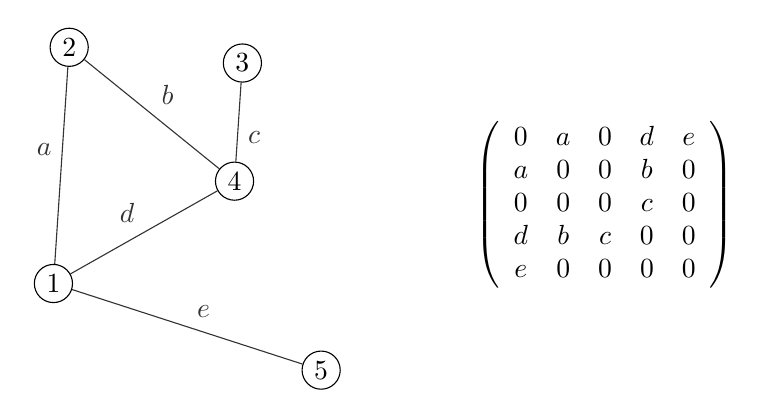
\begin{tikzpicture}[auto]
      \tikzstyle{every node} = [draw, circle, inner sep = 2pt]
      \node(1) at (1,2) {1};
      \node(2) at (1.2,5) {2};
      \node(3) at (3.4,4.8) {3};
      \node(4) at (3.3,3.3) {4};
      \node(5) at (4.4,0.9) {5};

      \tikzstyle{every node} = []
      \path[opacity=0.8]
      (1) edge node {$a$} (2);
      \path[opacity=0.8]
      (2) edge node {$b$} (4);
      \path[opacity=0.8]
      (4) edge node[swap] {$c$} (3);
      \path[opacity=0.8]
      (1) edge node {$d$} (4);
      \path[opacity=0.8]
      (1) edge node {$e$} (5);
      \node at (8,3) {$\left(\begin{array}{ccccc}
          0 & a & 0 & d & e\\
          a & 0 & 0 & b & 0\\
          0 & 0 & 0 & c & 0\\
          d & b & c & 0 & 0\\
          e & 0 & 0 & 0 & 0
        \end{array}\right)$};
    \end{tikzpicture}
  \end{center}
\caption{Example of a graph and its adjacency matrix}
\label{fig:graph}
\end{figure}